\sectionwithtoclink{Calibration of the Heston Model}

\subsection{The Data}
\label{sec:data-cleaning}
The data we're working with is 1 days closing data from 13.11.2019, giving us over 3700 \\$(\text{class}, \text{maturity}, \text{strike})$ combinations,
where by class we mean call or put. Before fitting anything to this data a little cleaning is of course due. I've chosen to use mid point as the
target price; this is non-trivial, as anything within the spread might be a fair price, and the tightness of the spread will depend on the liquidity in the option,
not to mention the complication of hidden orders in the book making gauging the actual fair price even more difficult. Nevertheless, I've chosen to use midpoint
while throwing out any quote non-compliant with no-arbitrage. No-arbitrage in this case is actually more strict than actual arbitrage in the market since we're
taking the trading costs out of the picture. We also don't want to accept too-wide spreads, as these will usually be stale orders/arb conditions in the market,
making them a bad estimate of an actual price. So what is actually done for each point in our data on the form $\text{data}_i=(\text{Class}_i,T_i,K_i,\text{Bid}_i,\text{Ask}_i,\text{Mid}_i)\quad \text{for} \,\, i\in\{1,..,N\}$
We filter by the following

\begin{itemize}
  \item drop 0-bids: drop if ( $\text{Bid}_i = 0$ )
  \item drop crossed spreads: drop if $( \text{Ask}_i \leq \text{Bid}_i )$
  \item minimum price: drop if  $\text{Mid}_i<0.5$
  \item too wide spread: drop if $(\text{Msk}_i-\text{Mid}_i)/\text{Mid}_i>0.5$
\end{itemize}
A thing we've not talked much about until this point is the risk-free rate, which we've assumed to be constant until this point. We'll
slightly relax this assumption and find the risk-free rates for each maturity as well as the continuously paid dividend yield $q$. We will
arrive at these by solving the following minimisation problem~\cite{DataHandeling}. Let 
$$J=\{(T,K)\in\mathbb{R}^2:\exists i,j\in\{1,...,N\} ,T_i=T_j=T,K_i=K_j=K,\text{Class}_i=\text{Put},\text{Class}_j=\text{Call}\}$$
more simply, the strike-maturity combinations for which we have both a call and a put price, where we will use the notation for put and call prices $P^M(T,K),C^M(T,K)$.
To make the following sum make sense, we also define 
\begin{align}
\mathcal{T}=\{T\in\mathbb{R}:\exists K\in\mathbb{R}, (T,K)\in J\}\\
\mathcal{K}(T)=\{K\in\mathbb{R}:(K,T)\in J\}
\end{align}
giving us the problem
\begin{align}
\min_{\{r_T\}_{T\in\mathcal{T}},q\geq0}\sum_{T\in\mathcal{T}}\sum_{K\in\mathcal{K}(T)}(C^M(T,K)-P^M(T,K)-S_0e^{-qT}+Ke^{-r_T T})^2
\end{align}
where $\#\mathcal{T}<\infty$
The solution to this problem gives us the risk-free rates and dividend yield which minimizes the violations of put-call
parity across available strikes and maturities. We solve this using the constrained non-linear least squares solver from the Python library scipy~\cite{scipy2020}.
This way of estimating brings another problem: if a maturity has no strike with both a put and a call on it, we don't
generate a risk-free rate. We are lucky enough not to have this problem in our dataset, but it should be kept in mind.
Applied to our dataset this yields the following per-maturity risk-free rates and dividend yield:

\begin{center}
\begin{tabular}{lcccccc}
\textbf{Maturity} & Dec-19 & Jan-20 & Feb-20 & Mar-20 & Apr-20 & Jun-20 \\
\hline
$r_T$ & 0.0163 & 0.0231 & 0.0214 & 0.0206 & 0.0213 & 0.0200 \\[6pt]
\textbf{Maturity} & Sep-20 & Oct-20 & Nov-20 & Dec-20 & Jun-21 & Dec-21 \\
\hline
$r_T$ & 0.0193 & 0.0198 & 0.0193 & 0.0189 & 0.0188 & 0.0186 \\[6pt]
\multicolumn{2}{l}{$q$} & \multicolumn{5}{l}{$0.0191$} \\
\end{tabular}
\end{center}

We also apply some extra ``best practice'' for options data cleaning, limiting ourselves to quotes which are usually most liquid:
\begin{itemize}
  \item Maturity window: keep $7~\text{days} \le T \le 2~\text{years}$.
  \item Forward log-moneyness window: keep $|\log(K/F_T)| \le 0.3$, where $F_T = S_0 e^{(r_T-q)T}$.
\end{itemize} 
As well as some additional arbitrage bounds~\cite{ContagiousMarkets}:
\begin{itemize}
  \item $\max(S_0 e^{-qT} - K e^{-r_T T}, 0) \le C \le S_0 e^{-qT}$
  \item   $\max(K e^{-r_T T} - S_0 e^{-qT}, 0) \le P \le K e^{-r_T T}$
\end{itemize}

\subsection{The Calibration Problem}
Given the option prices observed on a given day, the goal is to find the set of parameters which gives us the best fit to the data.
Since we are calibrating the model directly under the risk-neutral measure, the parameters cannot be estimated directly from the
underlying and must instead be calibrated to option prices/implied volatilities. For this purpose we will look at the general weighted least squares problem
$$\min_{\omega \in \Omega} \sum_{i=1}^{N}(w_i(y_i-f(x_i,\omega)))^2
$$
where $f$ is the functional form of our choice taking predictors $x_i$ (in our case specifying strike, maturity, etc.) and a parameter set $\omega$ that we are optimising over, $y_i$ being the target value and
$w(x)$ being an optional weighting letting us choose which $x$'s to ``prioritise'' in the problem. In our case we've chosen to look at the Heston model, giving us the functional form of the integrals derived
in earlier sections, and focus the fit on price deviations, using the squared deviations as the objective, giving us the more concrete problem:

$$\min_{\omega \in \Omega} \sum_{i=1}^{N}(w_i(C^M(T_i,K_i)-C(T_i,K_i,\omega)))^2
$$

where $T_i,K_i$ are the $i$th time-strike pair still in our dataset.
Here it should be noted that choosing both the weights and more generally the objective functions is non-trivial, other options
could be changing targets and looking at implied volatilities, looking at absolute deviations in prices, or looking at \%-deviations as we end up doing too, all these options possibly giving entirely different fits.
We also make a not completely arbitrary choice to look at call prices. To also include the put prices that we observe we use put-call parity, but then another problem appears: we'll have multiple data points to target.
Best practice here is to include the more liquid instrument, generally this will be the OTM options, meaning we simply throw away the ITM options, also for calibration.


Moving on to talk about weights, we'll be looking at two different weightings: uniform weights ($w_i=1$) and relative error weighting ($w_i=1/C^M_i$).

\begin{center}
\begin{tabular}{p{0.45\textwidth} p{0.45\textwidth}}
\textbf{Uniform weighting ($w_i = 1$)} & \textbf{Relative error weighting ($w_i = 1/C^M_i$)} \\[4pt]
\textit{Pros:} & \textit{Pros:} \\
Simple and parameter-free. &
Treats all options equally regardless of price level, a mispricing of $1$\% on a cheap OTM option counts the same as $1$\% on an expensive ITM option. \\[4pt]
\textit{Cons:} & \textit{Cons:} \\
Dominated by expensive options (deep ITM, long maturity), so the fit to cheap options, which carry a lot of information about the shape of the volatility smile, is sometimes worse. &
Generally prioritizes the fit of cheap OTM options, potentially at the expense of more expensive options that are often more liquid.
\end{tabular}
\end{center}

We will later compare the fits these two methods generate.
By inverting the remaining call prices to implied volatilities we get the following implied volatility surface:

\begin{figure}[H]
  \centering
  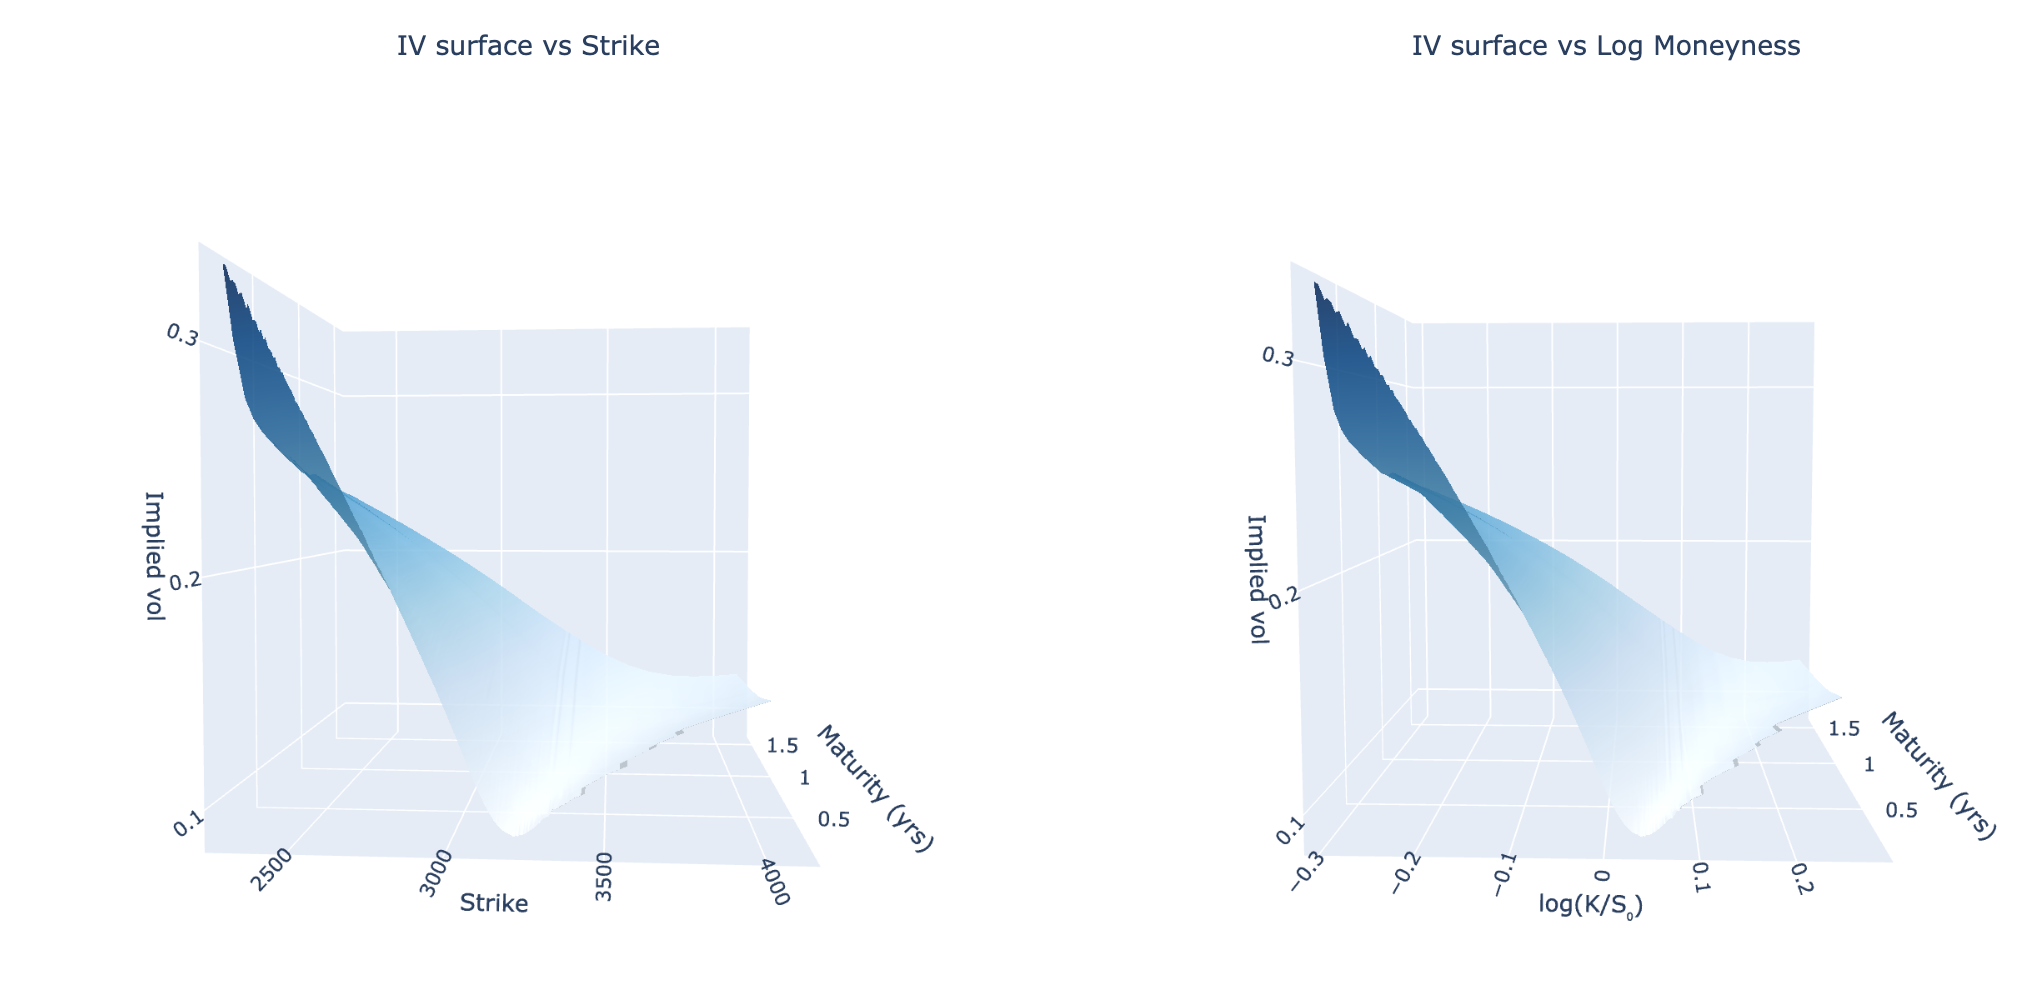
\includegraphics[width=\textwidth]{images/implied_vol_market_only.png}
  \caption{Market implied volatility surface from S\&P 500 options data (13 November 2019, $S_0 = 3094$) after data cleaning, arbitrage filtering, and OTM selection.}
  \label{fig:market-iv-surface}
\end{figure}

\subsection{Numerics}
Before we move on to talking about the calibration of the model to data and the actual fits, we should talk about how it's done. After moving through all the covered data cleaning steps
we want to solve the already discussed minimisation problem. This, however, means calculating a rather large number of integrals depending on the algorithm of choice, for this paper we will be using the ``Trust Region Reflective'' algorithm.
We need to calculate $N$ integrals simply
for evaluating the objective function, to calculate a numerical gradient means multiplying this by some $K > 2$. How hard it will be depends on the choice of quadrature  here the default choice for precision is the Gauss--Kronrod.
However, if speed is a priority, a different choice of quadrature speeds the computation time up significantly. Simply using the trapezoid rule on the interval $[0,400]$ with 4096 splits along with a bit of clever vectorisation in Python
allows us to significantly speed up calculation. To simply forget about anything above 400 seems fine, as we've already shown that the integrand is bounded by an exponential which will already basically have hit 0 at this point.
To showcase the speed increase I've set up a small experiment generating random parameter sets within the bounds:

\begin{center}
\begin{tabular}{lcc}
\textbf{Parameter} & \textbf{Lower} & \textbf{Upper} \\
\hline
$v_0$      & $0.05$ & $0.95$ \\
$\kappa$   & $0.50$ & $5.00$ \\
$\theta$   & $0.05$ & $0.95$ \\
$\sigma$      & $0.50$ & $0.95$ \\
$\rho$     & $-0.95$ & $-0.10$ \\
\end{tabular}
\end{center}

subject to the Feller condition $2\kappa\theta > \sigma^2$,
where we for each parameterset generate Call prices in a grid and try to fit using the different ways of integration. Before we run the experiment we'll add one more thing.
In~\cite{germano2017} they propose a way to calculate analytical gradients within the Heston model. They do this by finding a differentiable expression for the Heston CF and using differentiation under the integral sign to show that
\begin{equation}
\boldsymbol{\nabla} C= \frac{e^{-r\tau}}{\pi}\left[
\int_0^\infty \operatorname{Re}\!\left(\frac{e^{-iu\log\frac{K}{S_0}}}{iu}\,\boldsymbol{\nabla}\psi(u-i,\tau)\right)du
- K\int_0^\infty \operatorname{Re}\!\left(\frac{e^{-iu\log\frac{K}{S_0}}}{iu}\,\boldsymbol{\nabla}\psi(u,\tau)\right)du
\right]
\end{equation}
where $\boldsymbol{\theta}=(v_0,\theta,\rho,\kappa,\sigma)$. I would propose we can, by using their CF expression,
do the same but with the Lewis style formula. It is enough to show that $\frac{d}{d\theta_j}\frac{\Re(\psi(\theta,u,\tau)\cdot e^{-iku})}{\frac{1}{4}+u^2}$ is dominated by some function
$g(u)$ $\forall\theta_j\in\Theta_j$. The Germano et al.\ paper doesn't actually show this directly for their own formula, this also seems a bit out of scope for this paper, so I will simply
implement it and see if it works in the experiment.

\begin{equation}
\boldsymbol{\nabla} C = -\frac{e^{\frac{1}{2}k - rT}}{\pi}
\int_0^\infty \frac{\operatorname{Re}\!\left[e^{-iuk}\,\boldsymbol{\nabla}\psi\!\left(u-\tfrac{i}{2}\right)\right]}{u^2+\tfrac{1}{4}}\,du
\end{equation}
By using this analytical gradient we get to reduce the number of integral calculations when finding the gradient to simply 1 per parameter instead of the at least 2 needed to compute a numerical one.
Remember here that we are borrowing their version~\cite{germano2017} of the Heston CF as well as their partial derivatives. I've implemented this simply to see if it gives us any meaningful speed boost. I implement this
analytical gradient with both quadratures, so we actually get 4 different versions. The experiment will for each round report speed, objective score, and sum of absolute differences in the parameter space
from the solution found in the base case (Gauss--Kronrod) for each method.

\begin{figure}[H]
  \centering
  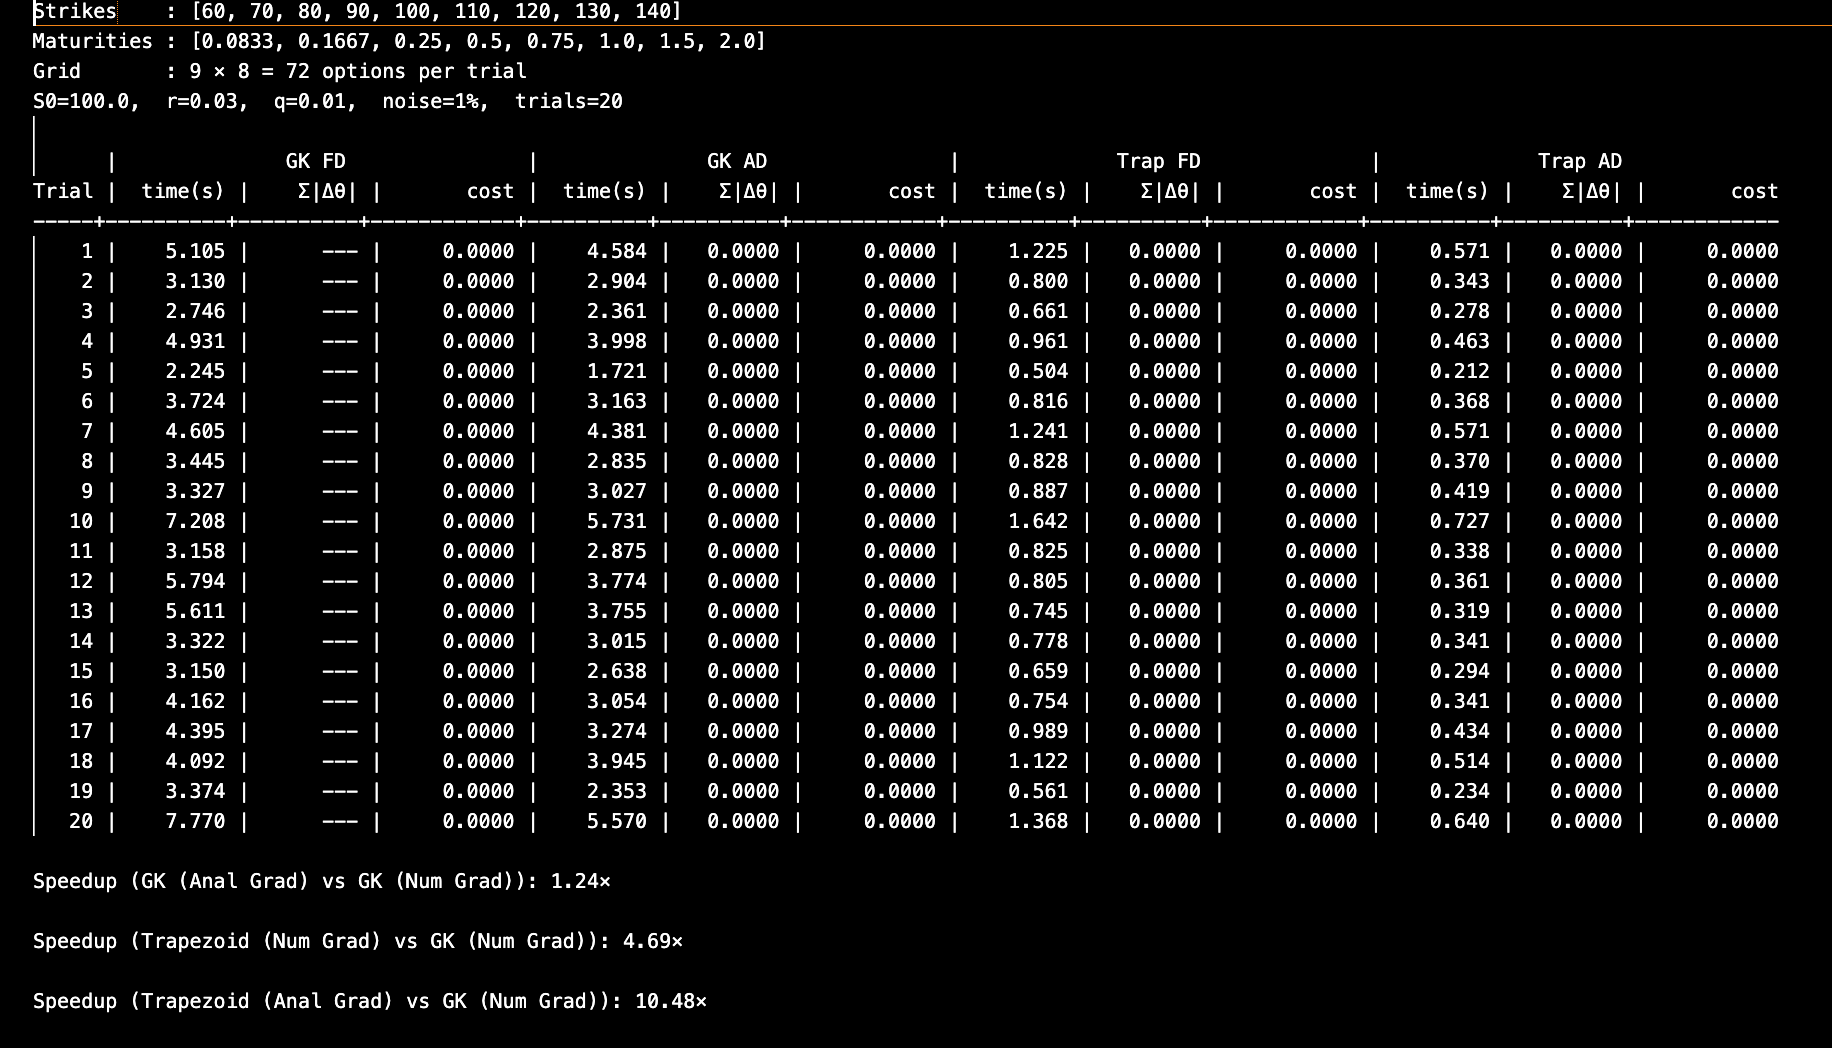
\includegraphics[width=0.9\textwidth]{images/calibration_speed_experiment.png}
  \caption{Calibration speed experiment: wait time and $\sum|\Delta\theta|$ relative to the GK baseline across 20 random Heston parameter draws satisfying the Feller condition. Code for replication can be found in the repo. We see convergence towards the true solution for all the methods, making time the only meaningfull measurement.}
  \label{fig:calibration-speed}
\end{figure}
From the experiment we see that the calibration for all 4 implementations seems to reach the same true minimum, or at least very close to it, and that
especially using the Trapezoid approach over the GK seems to speed us up quite a bit, giving us a 4.69x speed increase. For the GK we get an increase of 25\% from using the analytical gradient, which is of course still
a nice improvement yet less than I expected. Also way less than the 2x improvement we get when going from (Trapezoid -- num.\ diff.) $\rightarrow$ (Trapezoid -- anal.\ diff.), giving us a $\approx$10x speed-up in total.
Some of this improvement will most certainly be due to a better implementation of one or the other. Cutting the calibration to a tenth is still quite nice I think, especially in a situation where where speed matters more, 
imagine a situation where we try to keep a volatility surface generated by the live orderbook wanting to update it as often and quickly as possible. Well, anyway, for this project
speed is a non-issue, meaning we might as well take the slow approach that we know works. Going forward we'll simply use the GK approach with the numerical gradient, using the original Heston CF accounting for the LHT\cite{albrecher2007}.



\subsection{The calibration}
It's now time to calibrate to market data. We run our calibration with the initial guess
$$\omega_0 = (v_0,\kappa,\theta,\sigma,\rho) = (0.04,\ 2.0,\ 0.04,\ 0.4,\ -0.7)$$
once for each weighting getting parameter sets

\begin{center}
\begin{tabular}{lrrrrr}
\textbf{Weighting} & $v_0$ & $\kappa$ & $\theta$ & $\sigma$ & $\rho$ \\
\hline
Unweighted         & 0.0148 & 2.7212 & 0.0495 & 0.8778 & $-0.8290$ \\
Relative (\% error) & 0.0161 & 1.9856 & 0.0625 & 1.0506 & $-0.7648$ \\
\end{tabular}
\end{center}
Looking at the fits it's not hard to notice that they both violate the Feller condition. This however is not an uncommon occurrence when calibrating the Heston model,
and isn't a problem as it doesn't actually invalidate anything in the derivations done above.
Let's see how the implied volatility surfaces generated by these fits look compared to the market. The following surfaces are generated in the repository\cite{github_repo} and additional pictures may be found in the appendix.

\subsubsection{unweighted}

\begin{figure}[H]
  \centering
  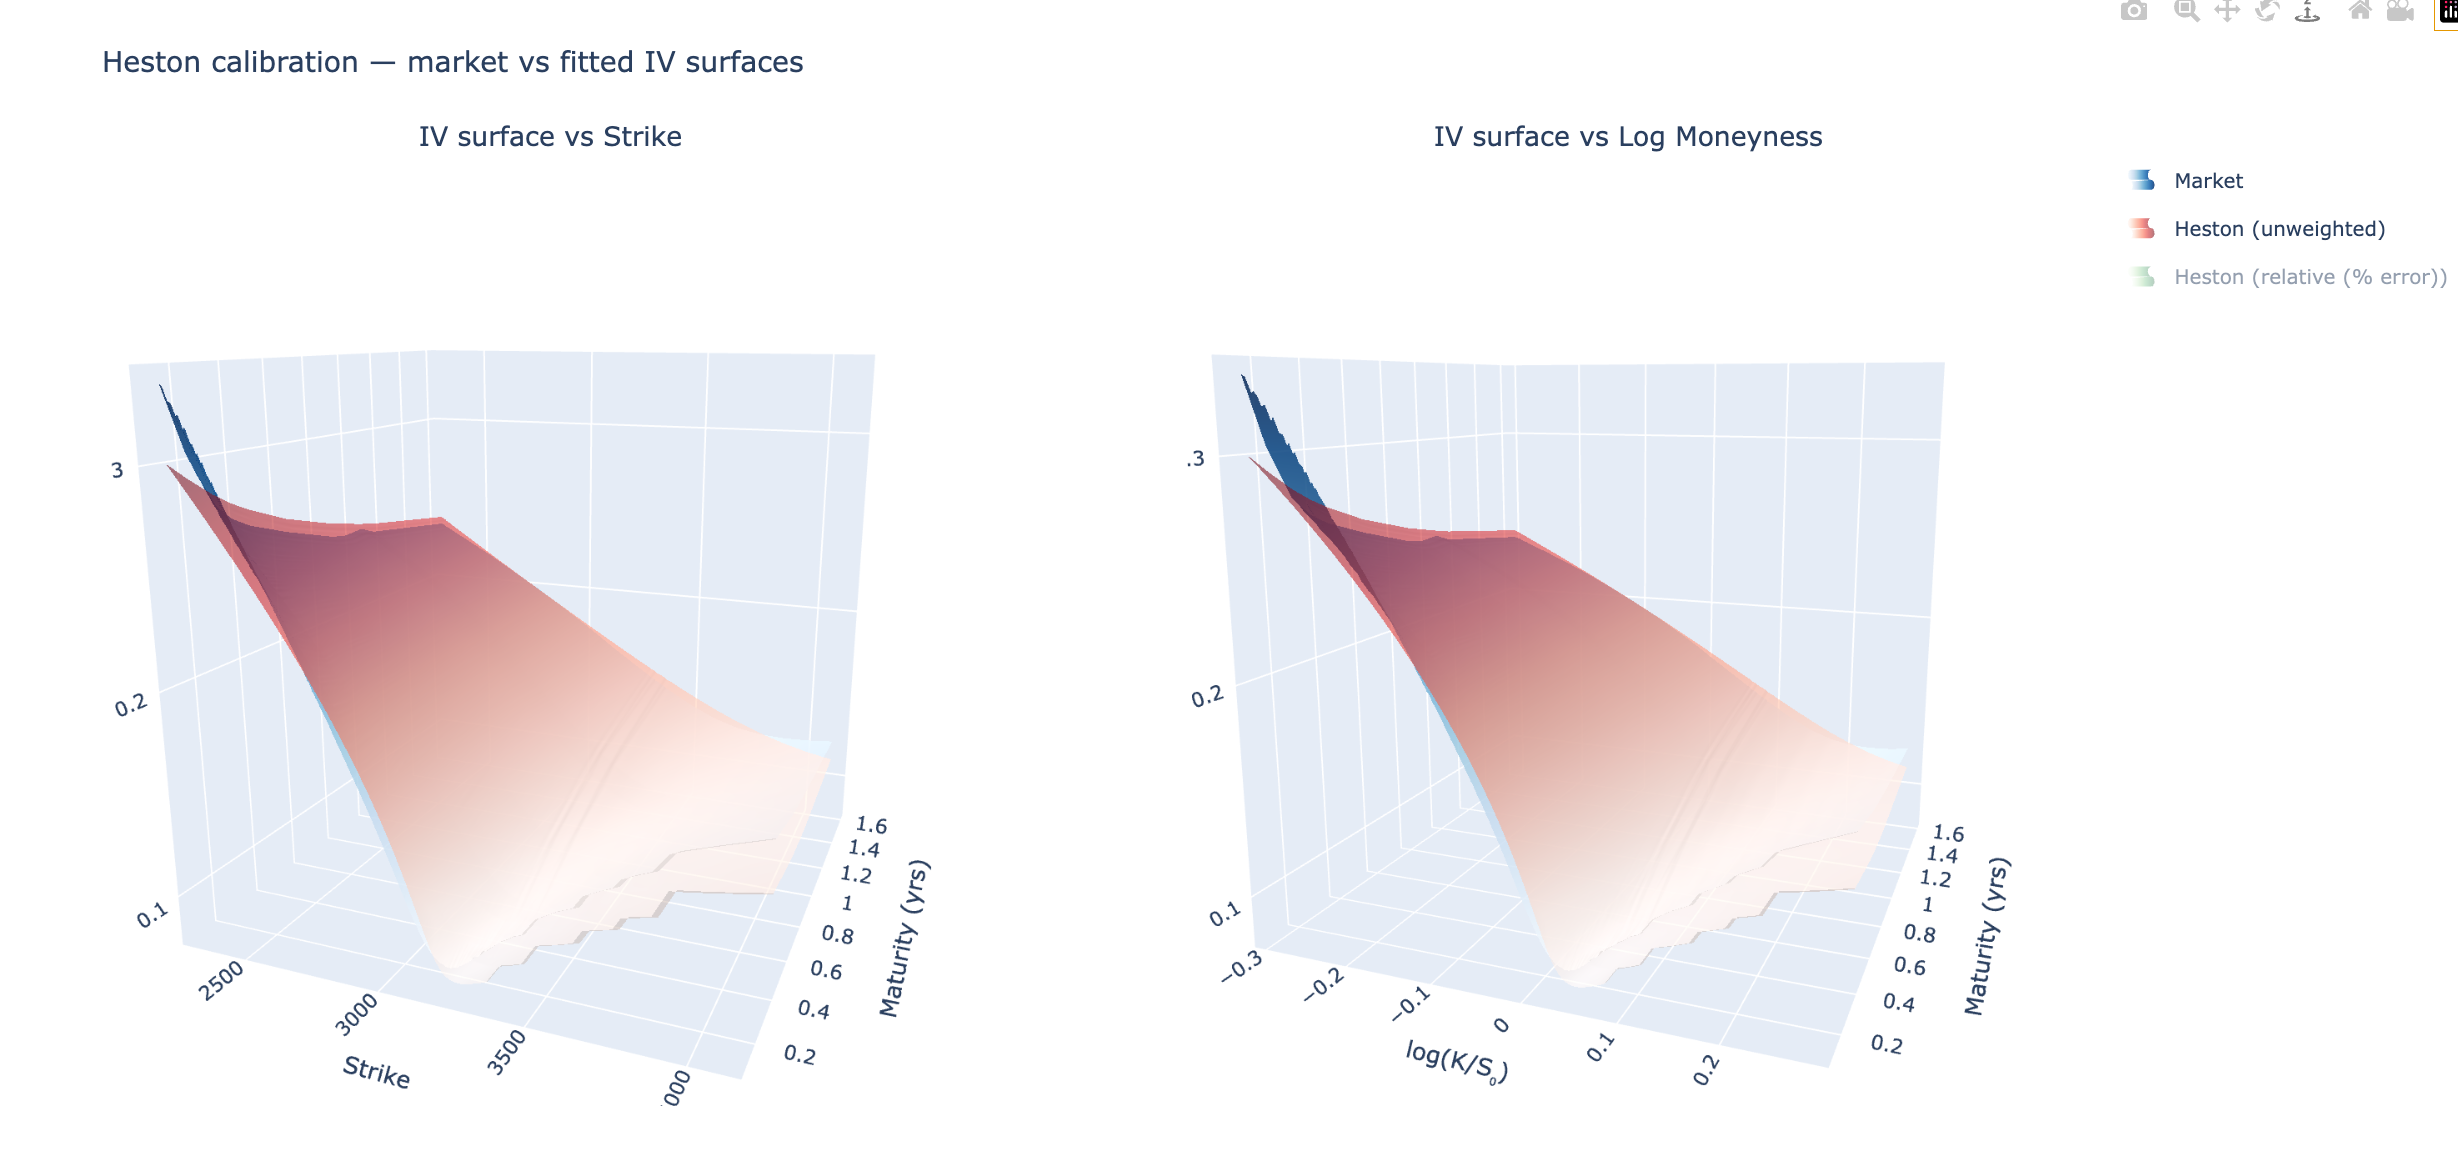
\includegraphics[width=\textwidth]{images/unweighted.png}
  \caption{Heston model fitted IV surface (unweighted calibration) vs.\ market implied volatility surface, S\&P 500 options (13 November 2019, $S_0 = 3094$).}
  \label{fig:iv-fit-unweighted}
\end{figure}

The fit seems to capture the overall shape of the surface quite well, especially on the ITM call side, while pricing OTM calls lower than the market.
This preference to fit the more expensive calls better is however something we expected and is simply a consequence of the choice of objective function.
However, on the very short maturities and low strikes we see that the market trades way higher than the model expects, indicating a higher demand for
deep ITM calls/far OTM puts than the model expects. When going further out on the curve we however see that the surfaces come closer and closer, giving
us a quite good fit on the longer maturity options (1--2 years).


\subsubsection{Relative error}

\begin{figure}[H]
  \centering
  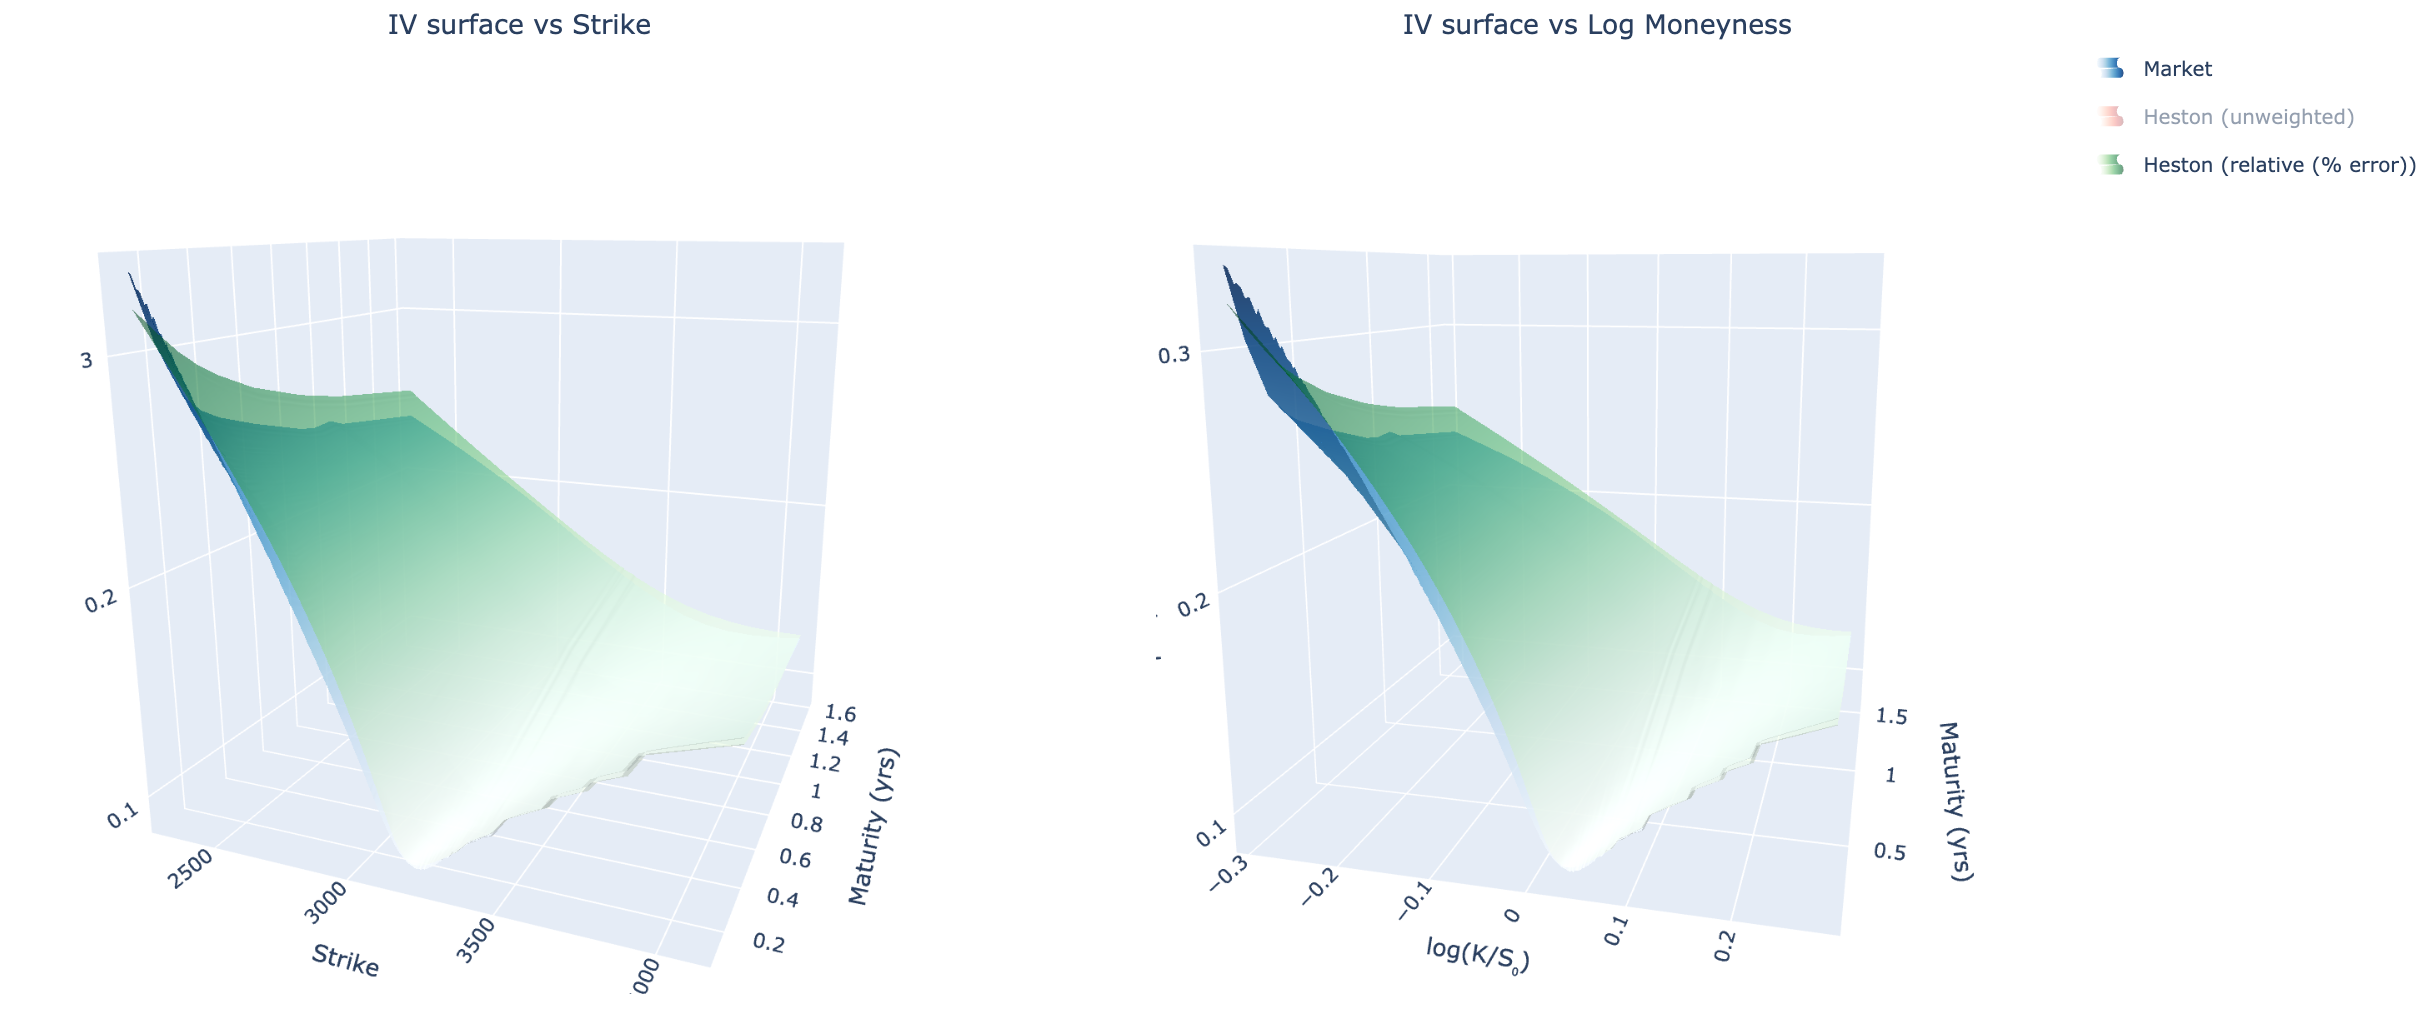
\includegraphics[width=\textwidth]{images/relative.png}
  \caption{Heston model fitted IV surface (relative error weighting) vs.\ market implied volatility surface, S\&P 500 options (13 November 2019, $S_0 = 3094$).}
  \label{fig:iv-fit-relative}
\end{figure}
Again the overall shape is quite good. However, where we before had fitted the ITM calls better, this time we are fitting the OTM side much better. We also see that we price the very short maturities quite well.
This however costs precision on the ITM call side, on longer maturities we are quite far off and never really seem to recover. So the short maturity and OTM sides are priced better. Well, these are for the most
part going to be the cheaper options where a small price error will mean a relatively big gain in the objective function.



To fit the implied volatility surface better we would probably need to switch objective functions into something penalizing errors in implied volatility directly like:
$$\sum_i w_i(\sigma_i^M-\sigma_i^{model})^2$$
this however would mean a worse fit on price, at least in the sum of squares sense, but is still the approach preferred by practitioners\footnote{I asked the options trader on the desk I work on.}.